% Options for packages loaded elsewhere
\PassOptionsToPackage{unicode}{hyperref}
\PassOptionsToPackage{hyphens}{url}
\PassOptionsToPackage{dvipsnames,svgnames,x11names}{xcolor}
%
\documentclass[
  11pt,
]{article}

\usepackage{amsmath,amssymb}
\usepackage{iftex}
\ifPDFTeX
  \usepackage[T1]{fontenc}
  \usepackage[utf8]{inputenc}
  \usepackage{textcomp} % provide euro and other symbols
\else % if luatex or xetex
  \usepackage{unicode-math}
  \defaultfontfeatures{Scale=MatchLowercase}
  \defaultfontfeatures[\rmfamily]{Ligatures=TeX,Scale=1}
\fi
\usepackage{lmodern}
\ifPDFTeX\else  
    % xetex/luatex font selection
\fi
% Use upquote if available, for straight quotes in verbatim environments
\IfFileExists{upquote.sty}{\usepackage{upquote}}{}
\IfFileExists{microtype.sty}{% use microtype if available
  \usepackage[]{microtype}
  \UseMicrotypeSet[protrusion]{basicmath} % disable protrusion for tt fonts
}{}
\makeatletter
\@ifundefined{KOMAClassName}{% if non-KOMA class
  \IfFileExists{parskip.sty}{%
    \usepackage{parskip}
  }{% else
    \setlength{\parindent}{0pt}
    \setlength{\parskip}{6pt plus 2pt minus 1pt}}
}{% if KOMA class
  \KOMAoptions{parskip=half}}
\makeatother
\usepackage{xcolor}
\usepackage[margin=0.75in]{geometry}
\setlength{\emergencystretch}{3em} % prevent overfull lines
\setcounter{secnumdepth}{-\maxdimen} % remove section numbering
% Make \paragraph and \subparagraph free-standing
\ifx\paragraph\undefined\else
  \let\oldparagraph\paragraph
  \renewcommand{\paragraph}[1]{\oldparagraph{#1}\mbox{}}
\fi
\ifx\subparagraph\undefined\else
  \let\oldsubparagraph\subparagraph
  \renewcommand{\subparagraph}[1]{\oldsubparagraph{#1}\mbox{}}
\fi

\usepackage{color}
\usepackage{fancyvrb}
\newcommand{\VerbBar}{|}
\newcommand{\VERB}{\Verb[commandchars=\\\{\}]}
\DefineVerbatimEnvironment{Highlighting}{Verbatim}{commandchars=\\\{\}}
% Add ',fontsize=\small' for more characters per line
\usepackage{framed}
\definecolor{shadecolor}{RGB}{241,243,245}
\newenvironment{Shaded}{\begin{snugshade}}{\end{snugshade}}
\newcommand{\AlertTok}[1]{\textcolor[rgb]{0.68,0.00,0.00}{#1}}
\newcommand{\AnnotationTok}[1]{\textcolor[rgb]{0.37,0.37,0.37}{#1}}
\newcommand{\AttributeTok}[1]{\textcolor[rgb]{0.40,0.45,0.13}{#1}}
\newcommand{\BaseNTok}[1]{\textcolor[rgb]{0.68,0.00,0.00}{#1}}
\newcommand{\BuiltInTok}[1]{\textcolor[rgb]{0.00,0.23,0.31}{#1}}
\newcommand{\CharTok}[1]{\textcolor[rgb]{0.13,0.47,0.30}{#1}}
\newcommand{\CommentTok}[1]{\textcolor[rgb]{0.37,0.37,0.37}{#1}}
\newcommand{\CommentVarTok}[1]{\textcolor[rgb]{0.37,0.37,0.37}{\textit{#1}}}
\newcommand{\ConstantTok}[1]{\textcolor[rgb]{0.56,0.35,0.01}{#1}}
\newcommand{\ControlFlowTok}[1]{\textcolor[rgb]{0.00,0.23,0.31}{#1}}
\newcommand{\DataTypeTok}[1]{\textcolor[rgb]{0.68,0.00,0.00}{#1}}
\newcommand{\DecValTok}[1]{\textcolor[rgb]{0.68,0.00,0.00}{#1}}
\newcommand{\DocumentationTok}[1]{\textcolor[rgb]{0.37,0.37,0.37}{\textit{#1}}}
\newcommand{\ErrorTok}[1]{\textcolor[rgb]{0.68,0.00,0.00}{#1}}
\newcommand{\ExtensionTok}[1]{\textcolor[rgb]{0.00,0.23,0.31}{#1}}
\newcommand{\FloatTok}[1]{\textcolor[rgb]{0.68,0.00,0.00}{#1}}
\newcommand{\FunctionTok}[1]{\textcolor[rgb]{0.28,0.35,0.67}{#1}}
\newcommand{\ImportTok}[1]{\textcolor[rgb]{0.00,0.46,0.62}{#1}}
\newcommand{\InformationTok}[1]{\textcolor[rgb]{0.37,0.37,0.37}{#1}}
\newcommand{\KeywordTok}[1]{\textcolor[rgb]{0.00,0.23,0.31}{#1}}
\newcommand{\NormalTok}[1]{\textcolor[rgb]{0.00,0.23,0.31}{#1}}
\newcommand{\OperatorTok}[1]{\textcolor[rgb]{0.37,0.37,0.37}{#1}}
\newcommand{\OtherTok}[1]{\textcolor[rgb]{0.00,0.23,0.31}{#1}}
\newcommand{\PreprocessorTok}[1]{\textcolor[rgb]{0.68,0.00,0.00}{#1}}
\newcommand{\RegionMarkerTok}[1]{\textcolor[rgb]{0.00,0.23,0.31}{#1}}
\newcommand{\SpecialCharTok}[1]{\textcolor[rgb]{0.37,0.37,0.37}{#1}}
\newcommand{\SpecialStringTok}[1]{\textcolor[rgb]{0.13,0.47,0.30}{#1}}
\newcommand{\StringTok}[1]{\textcolor[rgb]{0.13,0.47,0.30}{#1}}
\newcommand{\VariableTok}[1]{\textcolor[rgb]{0.07,0.07,0.07}{#1}}
\newcommand{\VerbatimStringTok}[1]{\textcolor[rgb]{0.13,0.47,0.30}{#1}}
\newcommand{\WarningTok}[1]{\textcolor[rgb]{0.37,0.37,0.37}{\textit{#1}}}

\providecommand{\tightlist}{%
  \setlength{\itemsep}{0pt}\setlength{\parskip}{0pt}}\usepackage{longtable,booktabs,array}
\usepackage{calc} % for calculating minipage widths
% Correct order of tables after \paragraph or \subparagraph
\usepackage{etoolbox}
\makeatletter
\patchcmd\longtable{\par}{\if@noskipsec\mbox{}\fi\par}{}{}
\makeatother
% Allow footnotes in longtable head/foot
\IfFileExists{footnotehyper.sty}{\usepackage{footnotehyper}}{\usepackage{footnote}}
\makesavenoteenv{longtable}
\usepackage{graphicx}
\makeatletter
\def\maxwidth{\ifdim\Gin@nat@width>\linewidth\linewidth\else\Gin@nat@width\fi}
\def\maxheight{\ifdim\Gin@nat@height>\textheight\textheight\else\Gin@nat@height\fi}
\makeatother
% Scale images if necessary, so that they will not overflow the page
% margins by default, and it is still possible to overwrite the defaults
% using explicit options in \includegraphics[width, height, ...]{}
\setkeys{Gin}{width=\maxwidth,height=\maxheight,keepaspectratio}
% Set default figure placement to htbp
\makeatletter
\def\fps@figure{htbp}
\makeatother

\makeatletter
\@ifpackageloaded{caption}{}{\usepackage{caption}}
\AtBeginDocument{%
\ifdefined\contentsname
  \renewcommand*\contentsname{Table of contents}
\else
  \newcommand\contentsname{Table of contents}
\fi
\ifdefined\listfigurename
  \renewcommand*\listfigurename{List of Figures}
\else
  \newcommand\listfigurename{List of Figures}
\fi
\ifdefined\listtablename
  \renewcommand*\listtablename{List of Tables}
\else
  \newcommand\listtablename{List of Tables}
\fi
\ifdefined\figurename
  \renewcommand*\figurename{Figure}
\else
  \newcommand\figurename{Figure}
\fi
\ifdefined\tablename
  \renewcommand*\tablename{Table}
\else
  \newcommand\tablename{Table}
\fi
}
\@ifpackageloaded{float}{}{\usepackage{float}}
\floatstyle{ruled}
\@ifundefined{c@chapter}{\newfloat{codelisting}{h}{lop}}{\newfloat{codelisting}{h}{lop}[chapter]}
\floatname{codelisting}{Listing}
\newcommand*\listoflistings{\listof{codelisting}{List of Listings}}
\makeatother
\makeatletter
\makeatother
\makeatletter
\@ifpackageloaded{caption}{}{\usepackage{caption}}
\@ifpackageloaded{subcaption}{}{\usepackage{subcaption}}
\makeatother
\ifLuaTeX
  \usepackage{selnolig}  % disable illegal ligatures
\fi
\usepackage{bookmark}

\IfFileExists{xurl.sty}{\usepackage{xurl}}{} % add URL line breaks if available
\urlstyle{same} % disable monospaced font for URLs
\hypersetup{
  pdftitle={Homework 2},
  pdfauthor={Nick Climaco},
  colorlinks=true,
  linkcolor={blue},
  filecolor={Maroon},
  citecolor={Blue},
  urlcolor={Blue},
  pdfcreator={LaTeX via pandoc}}

\title{Homework 2}
\author{Nick Climaco}
\date{February 9, 2024}

\begin{document}
\maketitle

\renewcommand*\contentsname{Table of contents}
{
\hypersetup{linkcolor=}
\setcounter{tocdepth}{3}
\tableofcontents
}
\newpage

\section{Chapter 3 Exercises (Hyndman and
Athanasopoulos)}\label{chapter-3-exercises-hyndman-and-athanasopoulos}

\begin{verbatim}
<Figure size 2700x1800 with 0 Axes>
\end{verbatim}

\begin{verbatim}
<Figure size 2700x1800 with 0 Axes>
\end{verbatim}

\subsection{Exercise 1}\label{exercise-1}

Consider the GDP information in global\_economy.

Plot the GDP per capita for each country over time. Which country has
the highest GDP per capita?

\begin{Shaded}
\begin{Highlighting}[]
\CommentTok{\# read in the data from R generated csv file}
\NormalTok{df\_global\_economy }\OperatorTok{=}\NormalTok{ pd.read\_csv(}\StringTok{"data/global\_economy.csv"}\NormalTok{, }
\NormalTok{                                parse\_dates}\OperatorTok{=}\NormalTok{[}\StringTok{"Year"}\NormalTok{], }
\NormalTok{                                index\_col}\OperatorTok{=}\NormalTok{[}\StringTok{"Year"}\NormalTok{])}

\NormalTok{df\_global\_economy[}\StringTok{"GDP\_Per\_Capita"}\NormalTok{] }\OperatorTok{=}\NormalTok{ (df\_global\_economy[}\StringTok{"GDP"}\NormalTok{] }\OperatorTok{/} 
\NormalTok{df\_global\_economy[}\StringTok{"Population"}\NormalTok{]).}\BuiltInTok{round}\NormalTok{(}\DecValTok{2}\NormalTok{)}

\CommentTok{\# calculate gdp per capita}
\NormalTok{df\_gdp\_per\_capita }\OperatorTok{=}\NormalTok{ df\_global\_economy[[}\StringTok{"Country"}\NormalTok{, }\StringTok{"GDP\_Per\_Capita"}\NormalTok{,}\StringTok{"GDP"}\NormalTok{, }\StringTok{"Population"}\NormalTok{]]}

\CommentTok{\#group by country}
\NormalTok{df\_grouped }\OperatorTok{=}\NormalTok{ df\_gdp\_per\_capita.groupby(}\StringTok{"Country"}\NormalTok{)}
\end{Highlighting}
\end{Shaded}

\subparagraph{Which country has the highest GDP per
capita?}\label{which-country-has-the-highest-gdp-per-capita}

\begin{Shaded}
\begin{Highlighting}[]
\CommentTok{\# sort vales of GDP per Capita by Country}
\NormalTok{df\_gdp\_per\_capita.groupby(}\StringTok{"Country"}\NormalTok{)[[}\StringTok{"GDP\_Per\_Capita"}\NormalTok{, }\StringTok{"GDP"}\NormalTok{, }\StringTok{"Population"}\NormalTok{]]}\OperatorTok{\textbackslash{}}
\NormalTok{  .}\BuiltInTok{max}\NormalTok{()}\OperatorTok{\textbackslash{}}
\NormalTok{    .reset\_index()}\OperatorTok{\textbackslash{}}
\NormalTok{      .sort\_values(}\StringTok{"GDP\_Per\_Capita"}\NormalTok{, ascending}\OperatorTok{=}\VariableTok{False}\NormalTok{)}\OperatorTok{\textbackslash{}}
\NormalTok{        .head(}\DecValTok{10}\NormalTok{)}
\end{Highlighting}
\end{Shaded}

\begin{longtable}[]{@{}lllll@{}}
\toprule\noalign{}
& Country & GDP\_Per\_Capita & GDP & Population \\
\midrule\noalign{}
\endhead
\bottomrule\noalign{}
\endlastfoot
163 & Monaco & 185152.53 & 7.060236e+09 & 38695.0 \\
139 & Liechtenstein & 179308.08 & 6.657171e+09 & 37922.0 \\
144 & Luxembourg & 119225.38 & 6.632734e+10 & 599449.0 \\
180 & Norway & 103059.25 & 5.235021e+11 & 5282223.0 \\
145 & Macao SAR, China & 94004.39 & 5.534800e+10 & 622567.0 \\
22 & Bermuda & 93605.75 & 6.109928e+09 & 65636.0 \\
202 & San Marino & 90682.58 & 2.752307e+09 & 33400.0 \\
114 & Isle of Man & 89941.64 & 7.428280e+09 & 84287.0 \\
197 & Qatar & 88564.82 & 2.062247e+11 & 2639211.0 \\
232 & Switzerland & 88415.63 & 7.091826e+11 & 8466017.0 \\
\end{longtable}

The country with the highest GDP per Capita is Monaca. It is a
city-state that borders the Mediterranean Sea. Moreover, looking at the
table we can infer that rich countries with very small population have
higher GDP per Capita which makes sense.

\subparagraph{How has this changed over
time?}\label{how-has-this-changed-over-time}

\begin{Shaded}
\begin{Highlighting}[]
\CommentTok{\# plot the time series}
\NormalTok{plt.figure(figsize}\OperatorTok{=}\NormalTok{(}\DecValTok{9}\NormalTok{,}\DecValTok{6}\NormalTok{))}

\NormalTok{sns.set\_style(}\StringTok{"whitegrid"}\NormalTok{)}

\CommentTok{\# create lines for each country}
\ControlFlowTok{for}\NormalTok{ country, value }\KeywordTok{in}\NormalTok{ df\_grouped:}
\NormalTok{    sns.lineplot(x}\OperatorTok{=}\NormalTok{value.index, }
\NormalTok{                 y }\OperatorTok{=} \StringTok{"GDP\_Per\_Capita"}\NormalTok{, }
\NormalTok{                 data}\OperatorTok{=}\NormalTok{value, label }\OperatorTok{=} \VariableTok{None}\NormalTok{)}

\CommentTok{\# add labels}
\NormalTok{plt.title(}\StringTok{\textquotesingle{}GDP per Capita Time Series by Country\textquotesingle{}}\NormalTok{)}
\NormalTok{plt.xlabel(}\StringTok{\textquotesingle{}Year\textquotesingle{}}\NormalTok{)}
\NormalTok{plt.ylabel(}\StringTok{\textquotesingle{}GDP per Capita\textquotesingle{}}\NormalTok{)}
\NormalTok{plt.grid()}
\NormalTok{plt.show()}
\end{Highlighting}
\end{Shaded}

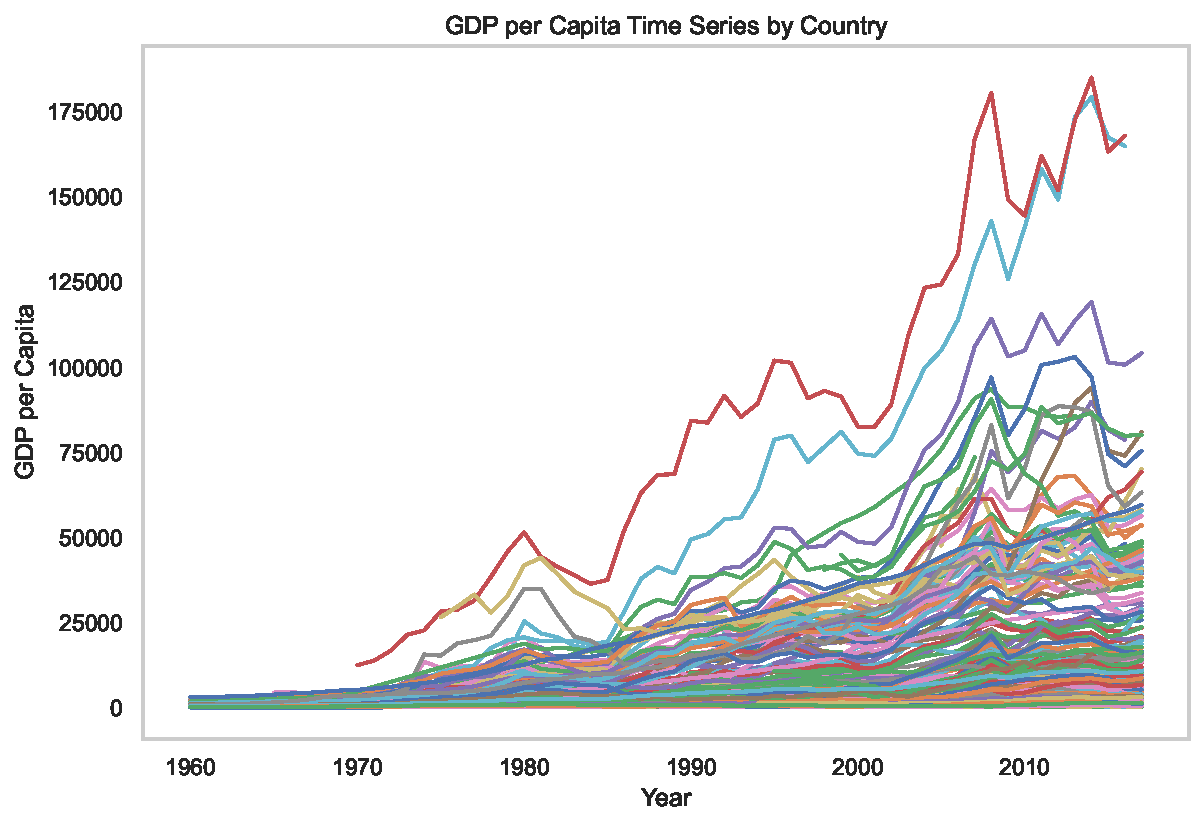
\includegraphics{hw2_files/figure-pdf/cell-5-output-1.pdf}

\subsection{Exercise 2}\label{exercise-2}

For each of the following series, make a graph of the data. If
transforming seems appropriate, do so and describe the effect.

\subparagraph{United States GDP from
global\_economy.}\label{united-states-gdp-from-global_economy.}

\begin{Shaded}
\begin{Highlighting}[]
\CommentTok{\# filter USA from the rest of the data}
\NormalTok{df\_us\_gdp }\OperatorTok{=}\NormalTok{ df\_global\_economy[df\_global\_economy[}\StringTok{"Country"}\NormalTok{] }\OperatorTok{==} \StringTok{"United States"}\NormalTok{]}
\end{Highlighting}
\end{Shaded}

\begin{Shaded}
\begin{Highlighting}[]
\CommentTok{\#plot}
\NormalTok{plt.figure(figsize}\OperatorTok{=}\NormalTok{(}\DecValTok{9}\NormalTok{,}\DecValTok{6}\NormalTok{))}

\NormalTok{sns.lineplot(x}\OperatorTok{=}\NormalTok{df\_us\_gdp.index, }
\NormalTok{             y }\OperatorTok{=}\NormalTok{ df\_us\_gdp.GDP)}

\CommentTok{\# edit labels}
\NormalTok{plt.xlabel(}\StringTok{"Year"}\NormalTok{)}
\NormalTok{plt.ylabel(}\StringTok{"Value (in $)"}\NormalTok{)}
\NormalTok{plt.title(}\StringTok{"US GDP"}\NormalTok{)}

\NormalTok{plt.show()}
\end{Highlighting}
\end{Shaded}

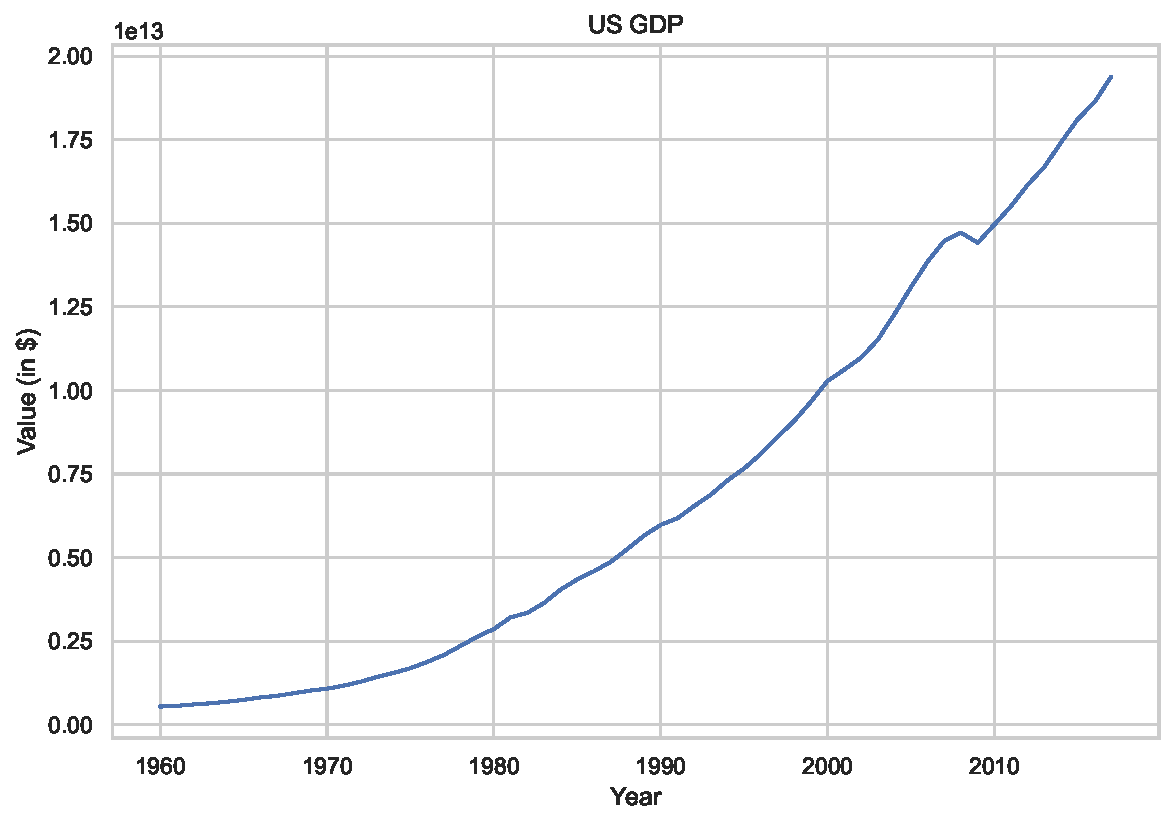
\includegraphics{hw2_files/figure-pdf/cell-7-output-1.pdf}

\subparagraph{Slaughter of Victorian ``Bulls, bullocks and steers'' in
aus\_livestock.}\label{slaughter-of-victorian-bulls-bullocks-and-steers-in-aus_livestock.}

\begin{Shaded}
\begin{Highlighting}[]
\CommentTok{\# read in data}
\NormalTok{df\_aus\_livestock }\OperatorTok{=}\NormalTok{ pd.read\_csv(}\StringTok{"aus\_livestock.csv"}\NormalTok{, }
\NormalTok{                               parse\_dates}\OperatorTok{=}\NormalTok{[}\StringTok{"Month"}\NormalTok{], }
\NormalTok{                               index\_col}\OperatorTok{=}\NormalTok{[}\StringTok{\textquotesingle{}Month\textquotesingle{}}\NormalTok{])}

\CommentTok{\# filter animal in animals}
\NormalTok{df\_filtered\_livestock }\OperatorTok{=}\NormalTok{ df\_aus\_livestock[df\_aus\_livestock[}\StringTok{"Animal"}\NormalTok{] }\OperatorTok{==} \OperatorTok{\textbackslash{}}
  \StringTok{"Bulls, bullocks and steers"}\NormalTok{]}

\NormalTok{df\_filtered\_livestock }\OperatorTok{=}\NormalTok{ df\_filtered\_livestock[[}\StringTok{"Count"}\NormalTok{]]}
\end{Highlighting}
\end{Shaded}

\begin{Shaded}
\begin{Highlighting}[]
\CommentTok{\# plot the time series}
\NormalTok{plt.figure(figsize}\OperatorTok{=}\NormalTok{(}\DecValTok{9}\NormalTok{,}\DecValTok{6}\NormalTok{))}

\NormalTok{sns.lineplot(x }\OperatorTok{=}\NormalTok{ df\_filtered\_livestock.index, }
\NormalTok{             y }\OperatorTok{=}\NormalTok{ df\_filtered\_livestock[}\StringTok{"Count"}\NormalTok{],}
\NormalTok{             errorbar}\OperatorTok{=}\VariableTok{None}\NormalTok{)}

\NormalTok{plt.xlabel(}\StringTok{"Month[1M]"}\NormalTok{)}
\NormalTok{plt.ylabel(}\StringTok{"Count"}\NormalTok{)}
\NormalTok{plt.title(}\StringTok{"Slaughter of Bulls, bullocks and steers in Australia"}\NormalTok{)}

\NormalTok{plt.show()}
\end{Highlighting}
\end{Shaded}

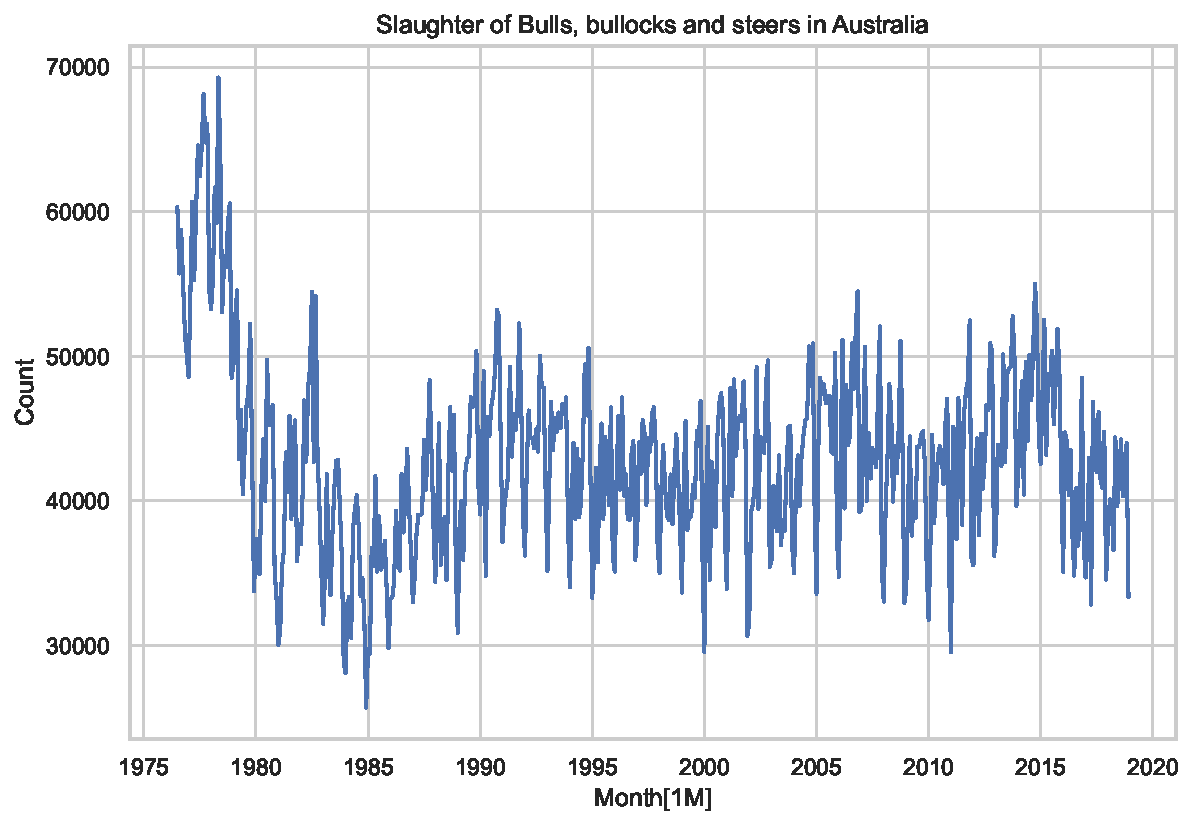
\includegraphics{hw2_files/figure-pdf/cell-9-output-1.pdf}

Looking the plot, we can see that the variation of the data is all over
place. To combat the we must imploy transformations in order to mitigate
the variability of the data.

Let us try a log tranform on the data and determine whether it is able
to reduce the variability on the data.

\begin{Shaded}
\begin{Highlighting}[]
\CommentTok{\# apply log transform}
\NormalTok{df\_filtered\_livestock[}\StringTok{"log\_Count"}\NormalTok{] }\OperatorTok{=}\NormalTok{ np.log(df\_filtered\_livestock[}\StringTok{"Count"}\NormalTok{] }\OperatorTok{+} \FloatTok{0.001}\NormalTok{)}
\end{Highlighting}
\end{Shaded}

\begin{Shaded}
\begin{Highlighting}[]
\NormalTok{plt.figure(figsize}\OperatorTok{=}\NormalTok{(}\DecValTok{9}\NormalTok{,}\DecValTok{6}\NormalTok{))}

\NormalTok{sns.lineplot(x }\OperatorTok{=}\NormalTok{ df\_filtered\_livestock.index, }
\NormalTok{             y }\OperatorTok{=}\NormalTok{ df\_filtered\_livestock[}\StringTok{"log\_Count"}\NormalTok{],}
\NormalTok{             errorbar}\OperatorTok{=}\VariableTok{None}\NormalTok{)}

\NormalTok{plt.xlabel(}\StringTok{"Month[1M]"}\NormalTok{)}
\NormalTok{plt.ylabel(}\StringTok{"Log\_Count"}\NormalTok{)}
\NormalTok{plt.title(}\StringTok{"Slaughter of Bulls, bullocks and steers in Australia"}\NormalTok{)}

\NormalTok{plt.show()}
\end{Highlighting}
\end{Shaded}

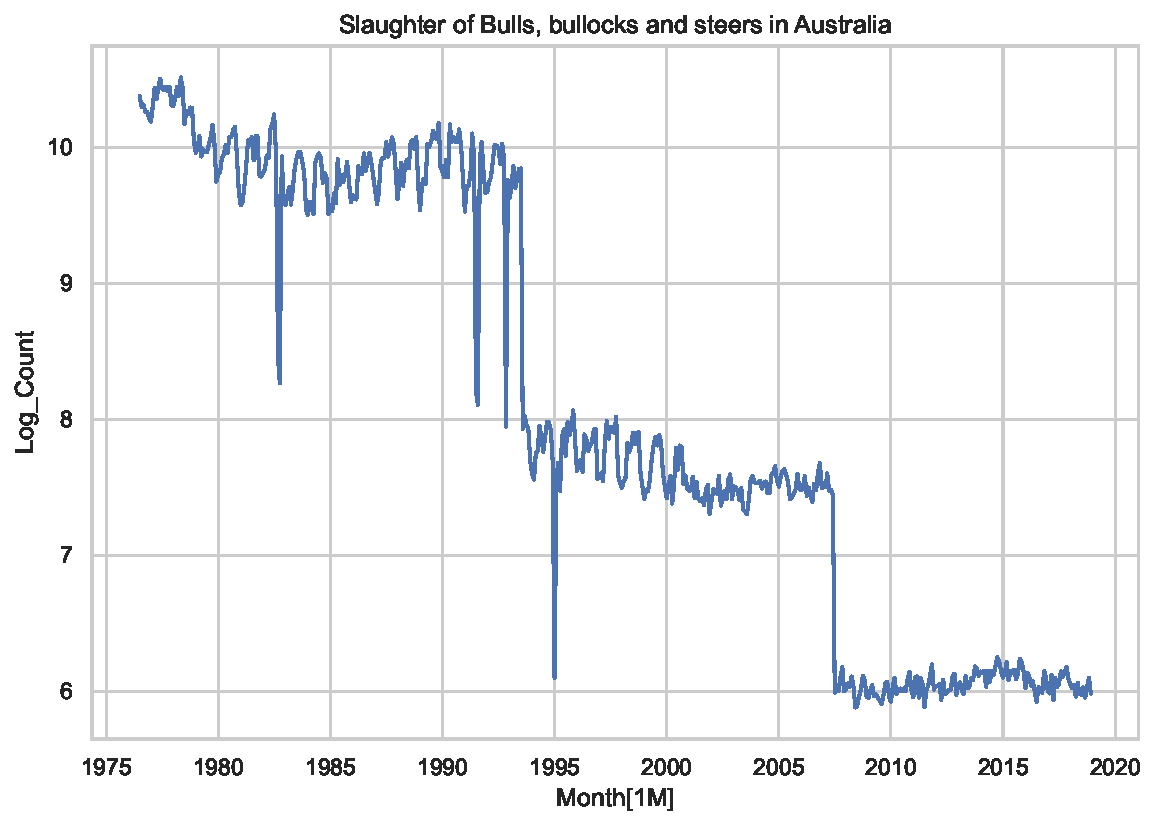
\includegraphics{hw2_files/figure-pdf/cell-11-output-1.pdf}

Log tranfrom did not quite create homogenous time series. Let's try some
other transformation

\n

\begin{Shaded}
\begin{Highlighting}[]
\ImportTok{from}\NormalTok{ scipy.stats }\ImportTok{import}\NormalTok{ boxcox}

\NormalTok{df\_filtered\_livestock[}\StringTok{"boxcox\_Count"}\NormalTok{], lambda\_val }\OperatorTok{=}\NormalTok{ boxcox(df\_filtered\_livestock[}\StringTok{"Count"}\NormalTok{] }\OperatorTok{+} \FloatTok{0.001}\NormalTok{)}
\end{Highlighting}
\end{Shaded}

\begin{Shaded}
\begin{Highlighting}[]
\NormalTok{plt.figure(figsize}\OperatorTok{=}\NormalTok{(}\DecValTok{9}\NormalTok{,}\DecValTok{6}\NormalTok{))}

\NormalTok{sns.lineplot(x }\OperatorTok{=}\NormalTok{ df\_filtered\_livestock.index, }
\NormalTok{             y }\OperatorTok{=}\NormalTok{ df\_filtered\_livestock[}\StringTok{"boxcox\_Count"}\NormalTok{], }
\NormalTok{             errorbar}\OperatorTok{=}\VariableTok{None}\NormalTok{)}

\NormalTok{plt.xlabel(}\StringTok{"Month[1M]"}\NormalTok{)}
\NormalTok{plt.ylabel(}\StringTok{"boxcox\_Count"}\NormalTok{)}
\NormalTok{plt.title(}\StringTok{"Slaughter of Bulls, bullocks and steers in Australia"}\NormalTok{)}

\NormalTok{plt.show()}
\end{Highlighting}
\end{Shaded}

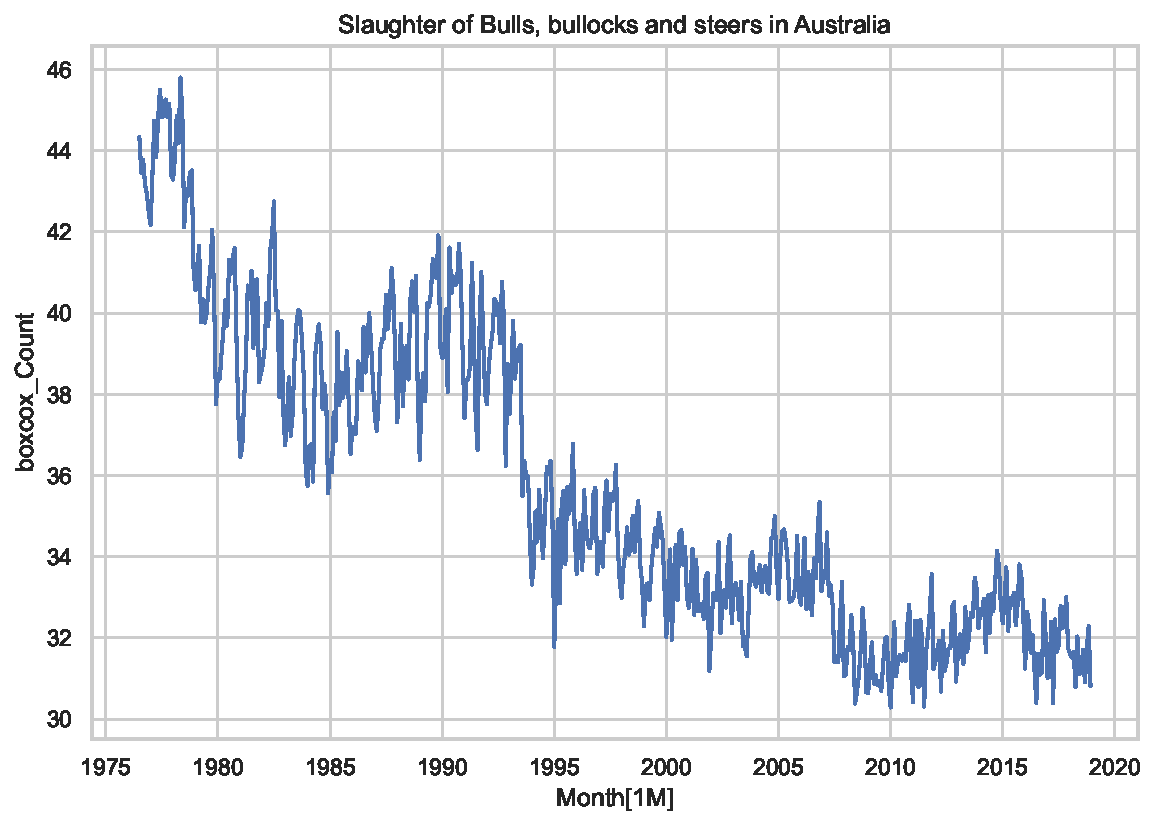
\includegraphics{hw2_files/figure-pdf/cell-13-output-1.pdf}

\subparagraph{Victorian Electricity Demand from
vic\_elec}\label{victorian-electricity-demand-from-vic_elec}

\begin{Shaded}
\begin{Highlighting}[]
\NormalTok{df\_vic\_elec }\OperatorTok{=}\NormalTok{ pd.read\_csv(}\StringTok{"vic\_elec.csv"}\NormalTok{, parse\_dates}\OperatorTok{=}\NormalTok{[}\StringTok{"Time"}\NormalTok{], index\_col }\OperatorTok{=}\NormalTok{ [}\StringTok{"Time"}\NormalTok{])}
\NormalTok{df\_demand }\OperatorTok{=}\NormalTok{ df\_vic\_elec[[}\StringTok{"Demand"}\NormalTok{]]}
\end{Highlighting}
\end{Shaded}

\begin{Shaded}
\begin{Highlighting}[]
\NormalTok{plt.plot(df\_demand.index, df\_demand[}\StringTok{"Demand"}\NormalTok{])}

\NormalTok{plt.xlabel(}\StringTok{"Time[30mins]"}\NormalTok{)}
\NormalTok{plt.ylabel(}\StringTok{"Demand of Electicity"}\NormalTok{)}
\NormalTok{plt.title(}\StringTok{"Electricity Demand"}\NormalTok{)}

\NormalTok{plt.show()}
\end{Highlighting}
\end{Shaded}

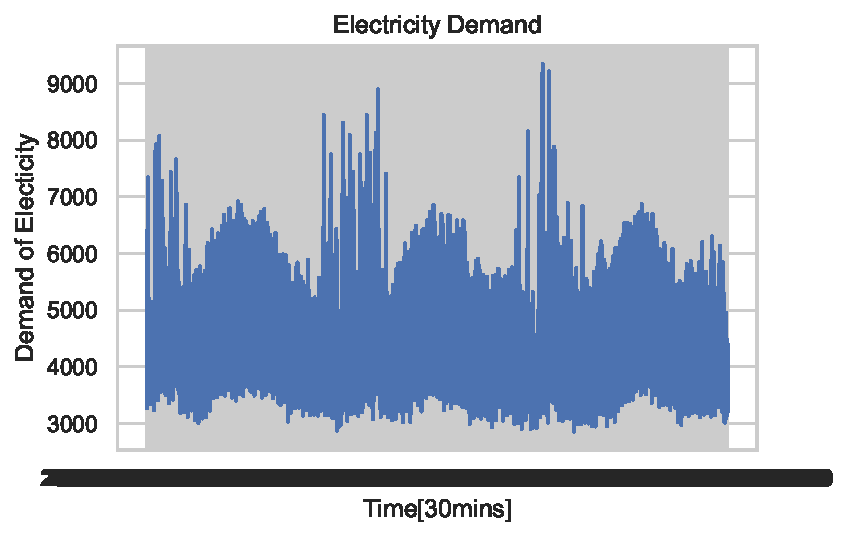
\includegraphics{hw2_files/figure-pdf/cell-15-output-1.pdf}

\begin{Shaded}
\begin{Highlighting}[]
\NormalTok{df\_demand[}\StringTok{\textquotesingle{}boxcox\_Demand\textquotesingle{}}\NormalTok{], \_  }\OperatorTok{=}\NormalTok{ boxcox(df\_demand[}\StringTok{\textquotesingle{}Demand\textquotesingle{}}\NormalTok{])}

\NormalTok{plt.plot(df\_demand.index, df\_demand[}\StringTok{"boxcox\_Demand"}\NormalTok{])}

\NormalTok{plt.xlabel(}\StringTok{"Time[30mins]"}\NormalTok{)}
\NormalTok{plt.ylabel(}\StringTok{"BoxCox Demand"}\NormalTok{)}
\NormalTok{plt.title(}\StringTok{"Electricity Demand (BoxCox)"}\NormalTok{)}

\NormalTok{plt.show()}
\end{Highlighting}
\end{Shaded}

\begin{verbatim}
C:\Users\nickc\AppData\Local\Temp\ipykernel_29956\1868045798.py:1: SettingWithCopyWarning: 
A value is trying to be set on a copy of a slice from a DataFrame.
Try using .loc[row_indexer,col_indexer] = value instead

See the caveats in the documentation: https://pandas.pydata.org/pandas-docs/stable/user_guide/indexing.html#returning-a-view-versus-a-copy
  df_demand['boxcox_Demand'], _  = boxcox(df_demand['Demand'])
\end{verbatim}

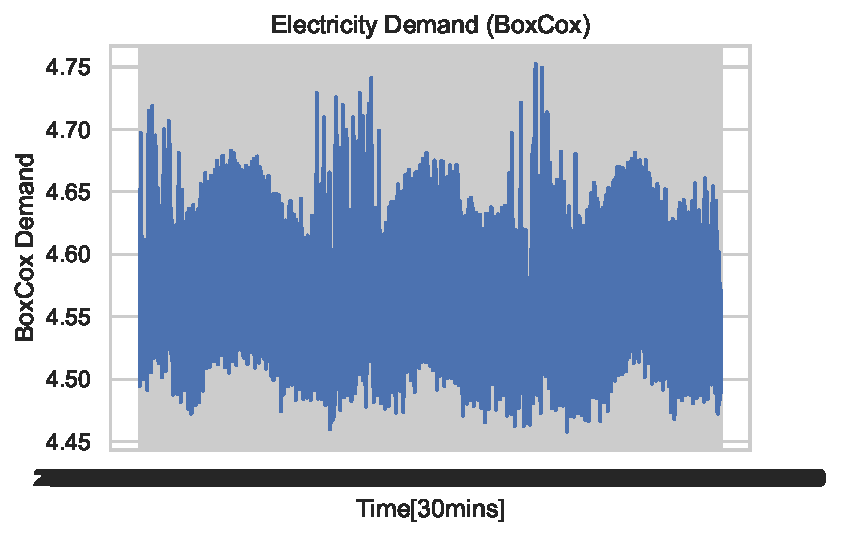
\includegraphics{hw2_files/figure-pdf/cell-16-output-2.pdf}

\subparagraph{Gas production from
aus\_production.}\label{gas-production-from-aus_production.}

\begin{Shaded}
\begin{Highlighting}[]
\NormalTok{df\_aus\_prod }\OperatorTok{=}\NormalTok{ pd.read\_csv(}\StringTok{"aus\_production.csv"}\NormalTok{, parse\_dates}\OperatorTok{=}\NormalTok{[}\StringTok{"Quarter"}\NormalTok{], index\_col}\OperatorTok{=}\NormalTok{[}\StringTok{\textquotesingle{}Quarter\textquotesingle{}}\NormalTok{])}
\NormalTok{df\_aus\_prod.head()}
\end{Highlighting}
\end{Shaded}

\begin{verbatim}
C:\Users\nickc\AppData\Local\Temp\ipykernel_29956\776626471.py:1: UserWarning: Could not infer format, so each element will be parsed individually, falling back to `dateutil`. To ensure parsing is consistent and as-expected, please specify a format.
  df_aus_prod = pd.read_csv("aus_production.csv", parse_dates=["Quarter"], index_col=['Quarter'])
\end{verbatim}

\begin{longtable}[]{@{}llllllll@{}}
\toprule\noalign{}
& Unnamed: 0 & Beer & Tobacco & Bricks & Cement & Electricity & Gas \\
Quarter & & & & & & & \\
\midrule\noalign{}
\endhead
\bottomrule\noalign{}
\endlastfoot
1956 Q1 & 1 & 284 & 5225.0 & 189.0 & 465 & 3923 & 5 \\
1956 Q2 & 2 & 213 & 5178.0 & 204.0 & 532 & 4436 & 6 \\
1956 Q3 & 3 & 227 & 5297.0 & 208.0 & 561 & 4806 & 7 \\
1956 Q4 & 4 & 308 & 5681.0 & 197.0 & 570 & 4418 & 6 \\
1957 Q1 & 5 & 262 & 5577.0 & 187.0 & 529 & 4339 & 5 \\
\end{longtable}

\begin{Shaded}
\begin{Highlighting}[]
\NormalTok{df\_beer }\OperatorTok{=}\NormalTok{ df\_aus\_prod[[}\StringTok{\textquotesingle{}Beer\textquotesingle{}}\NormalTok{]]}

\NormalTok{plt.plot(df\_beer.index, }\StringTok{\textquotesingle{}Beer\textquotesingle{}}\NormalTok{, data }\OperatorTok{=}\NormalTok{ df\_beer)}

\NormalTok{plt.xlabel(}\StringTok{\textquotesingle{}Quarter[1Q]\textquotesingle{}}\NormalTok{)}
\NormalTok{plt.ylabel(}\StringTok{\textquotesingle{}\# Produced\textquotesingle{}}\NormalTok{)}
\NormalTok{plt.title(}\StringTok{\textquotesingle{}Beer Production in Australia Per Quarter\textquotesingle{}}\NormalTok{)}

\NormalTok{n }\OperatorTok{=} \DecValTok{15}
\NormalTok{ticks }\OperatorTok{=}\NormalTok{ plt.xticks()[}\DecValTok{0}\NormalTok{]}
\NormalTok{labels }\OperatorTok{=}\NormalTok{ [item.get\_text() }\ControlFlowTok{for}\NormalTok{ item }\KeywordTok{in}\NormalTok{ plt.gca().get\_xticklabels()]}
\NormalTok{plt.xticks(ticks[::n], labels[::n], rotation }\OperatorTok{=}\DecValTok{45}\NormalTok{)}

\NormalTok{plt.show()}
\end{Highlighting}
\end{Shaded}

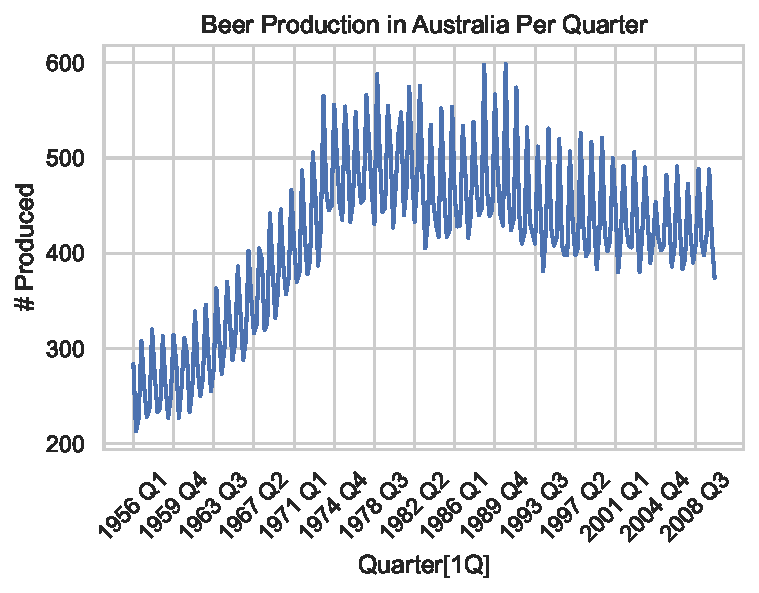
\includegraphics{hw2_files/figure-pdf/cell-18-output-1.pdf}

\subsection{Exercise 3}\label{exercise-3}

Why is a Box-Cox transformation unhelpful for the \texttt{canadian\_gas}
data?

\begin{Shaded}
\begin{Highlighting}[]
\NormalTok{df\_can\_gas }\OperatorTok{=}\NormalTok{ pd.read\_csv(}\StringTok{"canadian\_gas.csv"}\NormalTok{, parse\_dates}\OperatorTok{=}\NormalTok{[}\StringTok{\textquotesingle{}Month\textquotesingle{}}\NormalTok{], index\_col}\OperatorTok{=}\NormalTok{[}\StringTok{\textquotesingle{}Month\textquotesingle{}}\NormalTok{])}
\NormalTok{df\_can\_gas[}\StringTok{"boxcox\_Volume"}\NormalTok{],lmda }\OperatorTok{=}\NormalTok{ boxcox(df\_can\_gas[}\StringTok{"Volume"}\NormalTok{])}
\end{Highlighting}
\end{Shaded}

\begin{Shaded}
\begin{Highlighting}[]
\NormalTok{fig, ax }\OperatorTok{=}\NormalTok{ plt.subplots(nrows}\OperatorTok{=}\DecValTok{1}\NormalTok{, ncols}\OperatorTok{=}\DecValTok{2}\NormalTok{)}

\NormalTok{ax[}\DecValTok{0}\NormalTok{].plot(df\_can\_gas.index, df\_can\_gas[}\StringTok{\textquotesingle{}Volume\textquotesingle{}}\NormalTok{])}
\NormalTok{ax[}\DecValTok{0}\NormalTok{].set\_title(}\StringTok{\textquotesingle{}Original\textquotesingle{}}\NormalTok{)}
\NormalTok{ax[}\DecValTok{0}\NormalTok{].set\_xticklabels(ax[}\DecValTok{0}\NormalTok{].get\_xticks(), rotation}\OperatorTok{=}\DecValTok{45}\NormalTok{)}

\NormalTok{ax[}\DecValTok{1}\NormalTok{].plot(df\_can\_gas.index, df\_can\_gas[}\StringTok{\textquotesingle{}boxcox\_Volume\textquotesingle{}}\NormalTok{])}
\NormalTok{ax[}\DecValTok{1}\NormalTok{].set\_title(}\StringTok{\textquotesingle{}BoxCox Transformed\textquotesingle{}}\NormalTok{)}
\NormalTok{ax[}\DecValTok{1}\NormalTok{].set\_xticklabels(ax[}\DecValTok{1}\NormalTok{].get\_xticks(), rotation}\OperatorTok{=}\DecValTok{45}\NormalTok{)}
\NormalTok{plt.tight\_layout()}
\NormalTok{plt.show()}
\end{Highlighting}
\end{Shaded}

\begin{verbatim}
C:\Users\nickc\AppData\Local\Temp\ipykernel_29956\4111168296.py:5: UserWarning: set_ticklabels() should only be used with a fixed number of ticks, i.e. after set_ticks() or using a FixedLocator.
  ax[0].set_xticklabels(ax[0].get_xticks(), rotation=45)
C:\Users\nickc\AppData\Local\Temp\ipykernel_29956\4111168296.py:9: UserWarning: set_ticklabels() should only be used with a fixed number of ticks, i.e. after set_ticks() or using a FixedLocator.
  ax[1].set_xticklabels(ax[1].get_xticks(), rotation=45)
\end{verbatim}

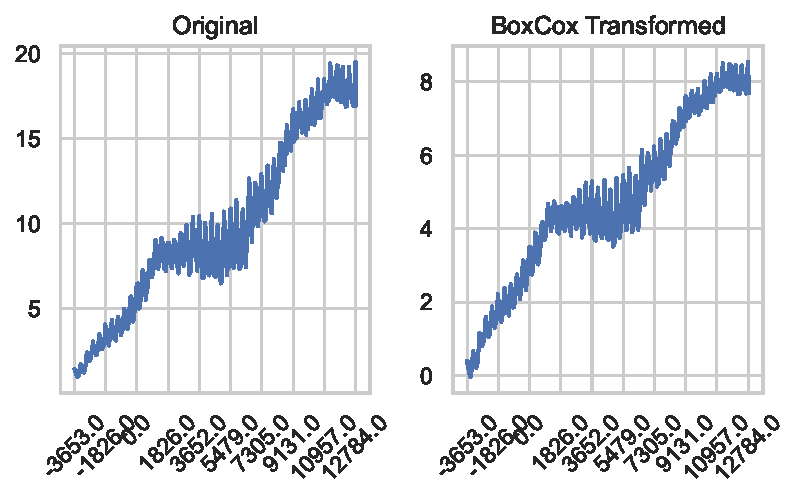
\includegraphics{hw2_files/figure-pdf/cell-20-output-2.pdf}

In this case, the boxcox transformation has little to no impact on the
variation of the time series which suggests that the original timeseries
already had a relativily constant or stable variation.

\subsection{Exercise 4}\label{exercise-4}

What Box-Cox transformation would you select for your retail data (from
Exercise 7 in Section 2.10)?

\subsection{Exercise 5}\label{exercise-5}

For the following series, find an appropriate Box-Cox transformation in
order to stabilise the variance. Tobacco from \texttt{aus\_production},
Economy class passengers between Melbourne and Sydney from
\texttt{ansett}, and Pedestrian counts at Southern Cross Station from
\texttt{pedestrian}.

\subsection{Exercise 7}\label{exercise-7}

Consider the last five years of the Gas data from
\texttt{aus\_production}.

\subparagraph{Plot the time series. Can you identify seasonal
fluctuations and/or a
trend-cycle?}\label{plot-the-time-series.-can-you-identify-seasonal-fluctuations-andor-a-trend-cycle}

\subparagraph{Use classical\_decomposition with type=multiplicative to
calculate the trend-cycle and seasonal
indices.}\label{use-classical_decomposition-with-typemultiplicative-to-calculate-the-trend-cycle-and-seasonal-indices.}

\subparagraph{Do the results support the graphical interpretation from
part
a?}\label{do-the-results-support-the-graphical-interpretation-from-part-a}

\subparagraph{Compute and plot the seasonally adjusted
data.}\label{compute-and-plot-the-seasonally-adjusted-data.}

\#\#\#\#\#Change one observation to be an outlier (e.g., add 300 to one
observation), and recompute the seasonally adjusted data. What is the
effect of the outlier?

\subparagraph{Does it make any difference if the outlier is near the end
rather than in the middle of the time
series?}\label{does-it-make-any-difference-if-the-outlier-is-near-the-end-rather-than-in-the-middle-of-the-time-series}

\subsection{Exercise 8}\label{exercise-8}

Recall your retail time series data (from Exercise 7 in Section 2.10).
Decompose the series using X-11. Does it reveal any outliers, or unusual
features that you had not noticed previously?

\subsection{Exercise 9}\label{exercise-9}

Figures 3.19 and 3.20 show the result of decomposing the number of
persons in the civilian labour force in Australia each month from
February 1978 to August 1995.

\subparagraph{Write about 3--5 sentences describing the results of the
decomposition. Pay particular attention to the scales of the graphs in
making your
interpretation.}\label{write-about-35-sentences-describing-the-results-of-the-decomposition.-pay-particular-attention-to-the-scales-of-the-graphs-in-making-your-interpretation.}

\subparagraph{Is the recession of 1991/1992 visible in the estimated
components?}\label{is-the-recession-of-19911992-visible-in-the-estimated-components}



\end{document}
